\section{Methodology}
\label{sec:urltran:method}
%
\URLTranSys seeks to use recent advances in natural language processing to improve the task of detecting phishing URLs.
Building \URLTranSys employs a two-pronged approach towards adapting transformers for the task of phishing URL detection.
First, state-of-the-art transformer models, BERT~\citep{devlin2019bert} and  RoBERTa~\citep{liu2019roberta}, are fine-tuned, starting from publicly available vocabularies and weights and across different hyperparameter settings and resulting in \URLTranSysb and \URLTranSysr, respectively.
Second, domain-specific vocabularies are built using different tokenization approaches, and a domain specific transformer (\URLTranSysc) is first pre-trained and then fine-tuned on the task. 

 The general architecture of all the explored models takes a three stage approach for inference shown in Figure~\ref{fig:urltran:transformer}. It first uses a subword tokenizer to extract tokens from a URL.
Next, a  transformer model generates an embedding vector for the unknown URL.
Finally, a classifier predicts a score indicating whether or not the unknown URL corresponds to a phishing web page.
\begin{figure}
	\centering
	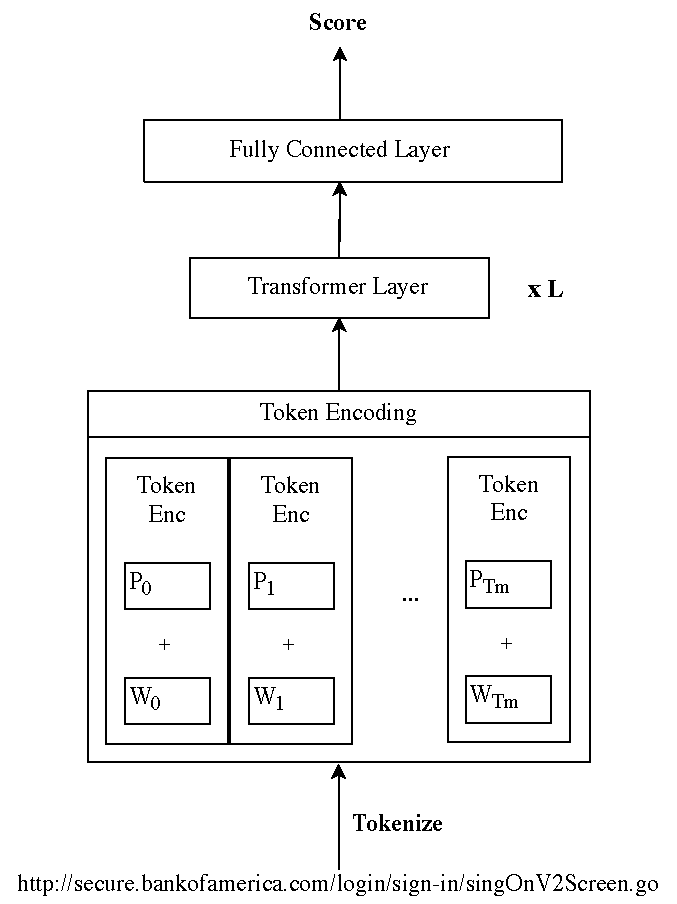
\includegraphics[width=0.4\linewidth]{urltran/figures/TransformerModel}
	\caption{\URLTranSys phishing URL detection model.}
	\label{fig:urltran:transformer}
\end{figure}
In the following sections, we first provide briefly summarize the transformer model architecture, followed by the training tasks used to train the model, and end with a description of the adversarial settings under which the best \URLTranSys model is evaluated and then trained with adversarial examples to improve its robustness.

\subsection{Architecture}
We describe the tokenization schemes and overall architecture for classification in this section, skipping a detailed description of transformer models for brevity.
Interested readers can review the transformer~\citep{vaswani2017attention}, BERT~\cite{devlin2019bert}, or RoBERTa~\citep{liu2019roberta} papers for details of the internal structure of transformer layers.

\subsubsection{Tokenization}
\label{sec:urltran:architecture:tokenization}
%
The raw input to the \URLTranSys model is the URL, which can be viewed as a text sequence.
The first step in the phishing URL detection task involves converting this input URL into a numerical vector which can be further processed by a classic machine learning or deep learning model.
Previous URL detection models~\citep{blum2020lexical} extracted lexical features by first splitting the URL with a set of important delimiters (e.g., `=', `/', `?', `.', ` ') and then creating a sparse binary features based on these tokens.
Recent deep learning-based URL detection models~\citep{le2018malicious,tajaddodianfar2020texception} instead include separate word-level and character-level CNNs where the character-level CNNs span different lengths of character subsequences.

Instead of these approaches, we experiment with multiple subword tokenization schemes in \URLTranSys.
Subword models have seen increased adoption in different tasks in NLP, including machine translation~\citep{sennrich2016neural}, word analogy~\citep{bojanowski2017enriching}, and question answering~\citep{zhang2019effective}.
Using subword models helps balance between the tradeoffs of using full-length words for each token (leading to fewer tokens required per input but a large token vocabulary) and character-based models (more tokens required per input but a smaller token vocabulary).
%allowing more input to be processed by a fixed-length model, 
%Using a subword model can provide morphological insights to improve inference.
For example, a full-length model would consider `bankofamerica' and `bankofcanada' as completely unrelated tokens, whereas a subword model can recognize the shared subword `bank' to correlate URLs belonging to the two banks.
Frequently occurring character substrings tend to correspond to subwords; common prefixes and suffixes can also provide relevant information.
%while being more robust to polymorphic attacks.
In particular, for fine-tuned \URLTranSysb and \URLTranSysr, we use the corresponding existing word piece~\citep{wu2016googles,devlin2019bert}  and Byte Pair Encoding (BPE) models~\citep{ratdford2019gpt2,liu2019roberta}, respectively.
In addition to these, we create custom character-level and byte-level BPE vocabularies using the training URL data to have a domain specific vocabulary for \URLTranSysc.
We test two different vocabulary sizes, 1K and 10K.
We tested  both sentence piece and BPE tokenization schemes in our models.
%as they attempt to find a balance of using both character substrings and full words and can capture unexpected unicode characters using their byte-level decomposition.


The BPE models first break the $m^{th}$ URL, $u_m$, into a sequence of text tokens, $\mathbf{TOK}_m$, where the individual tokens  may represent entire words or subwords~\citep{schuster2012japanese,sennrich2016neural,wu2016googles}.
Following the notation in~\cite{devlin2019bert}, the token sequence is formed as:
\begin{equation}
	\begin{split}
		& \mathbf{TOK}_m = \text{Tokenizer}(u_m)\\
	\end{split}
\label{eq:urltran:tok}
\end{equation}
%\end{comment}
\noindent where $\mathbf{TOK}_m$ is of length $T_m$ positions and consists of individual tokens ${Tok}_m^t$ at each position index $t$.
%${Tok}_t$ is an individual token generated from the $m^{th}$ URL generated by the wordpiece model.
For example, the BERT wordpiece token sequence generated from the URL of a popular banking login page,\\
\mbox{\small{$u_m$ = secure.bankofamerica.com/login/sign-in/signOnV2Screen.go}} \\
 is shown in Table~\ref{tab:urltran:boa}. The wordpiece model includes special text tokens specified by (\#\#) which build
 upon the previous token in the sequence. In the example in Table~\ref{tab:urltran:boa}, `\#\#of' refers to the continuation from s
 token (`bank'), and helps distinguish from the more common  separate token `of'.

\begin{table}
\centering
\resizebox{\linewidth}{!}{
\begin{tabular}{ll}
\hline
URL ($u_m$) & secure.bankofamerica.com/login/sign-in/signOnV2Screen.go \\
\hline
Token Sequence ($\mathbf{{TOK}_m}$) & \{ `secure', `.', `bank', `\#\#of', `\#\#ame', `\#\#rica', `.', `com', `/', `log', `\#\#in', `/', \\  & `sign', `-', `in', `/', `sign', `\#\#on', `\#\#v', `\#\#2', `\#\#screen', `.', `go' \} \\
  \hline
\end{tabular}
}
\caption{Example of the wordpiece token sequence extraction from a popular banking web page.}
\label{tab:urltran:boa}
\end{table}

\subsubsection{Classifier}
%
The final encoding produced by the transformer model can be used for a variety of downstream NLP tasks such
as language understanding, language inference, and question answering, and text classification.
We use the transformer embeddings for two tasks: pre-training masked language models, and fine-tuning for classification of phishing URLs.
Both of these tasks require a final representation layer which can be applied to multiple tokens for masked token prediction, and a pooled representation for classification.
The transformer models that we train use a single, dense two-class classification layer, which is applied to a special pooled token (`\texttt{[CLS]}') for classification. A dense layer having an output size equal to the size of the vocabulary of the tokenizer (\texttt{vocab\_size}) classes is used for predicting the masked token for the masked language modeling task during pre-training:

\begin{align}
	s_m = \sigma(\rmW_{p} \rvx_m^0 + \rvb_p) \label{eq:urltran:denseout}\\
	\rvs_m^t = \bm{\sigma} (\rmW_{v} \rvx_m^t + \rvb_v) \label{eq:urltran:denseword}
    %\label{eq:dense}
\end{align}

\noindent  In~(\ref{eq:urltran:denseout}), $\rmW_{p}$ and $\rvb$ are the weight matrix, bias vector respectively, for the final
dense linear layer for predicting the phising label.
$\sigma$ is the softmax function and 
 $s_m$ is the
score which predicts if the URL $\mathbf{u}_m$ corresponds to a phishing web page when performing classification.
Similarly, in~(\ref{eq:urltran:denseword}),
$\rvs_m^t, t \in [n]$ are 
 the sequence of masked token probability score vectors when performing masked language modeling for input token $\rvx_m^t$ computed using the softmax function $\bm{\sigma}$, with weight matrix $\rmW_{v}$ and bias vector $\rvb_v$.
 We now describe how input tokens are modified for masked language modeling and fine tuning.

\subsection{Training}
%
\subsubsection{Masked Language Modeling (MLM)}
The MLM task is commonly used to perform pre-training for transformers~\cite{devlin2019bert,liu2019roberta}. In this task, a random subset of tokens is replaced by a special `\texttt{[MASK]}' token.
 The training objective for the task is the cross-entropy loss corresponding to predicting the correct tokens at masked positions.
 The intuition for using this task for URLs is that specific query parameters and paths are generally associated with non-phishing URLs and therefore predicting masked tokens would help to uncover these associations.
 Similar intuitions derived from the cloze task~\cite{taylor1953cloze} motivate the usage of MLMs for pre-training natural language models.
Following the MLM hyperparameter settings for BERT, we selected 15\% of the tokens sampled uniformly for masking, of which 80\% are replaced, 10\% were left unchanged, and 10\% were replaced by a random vocabulary token at each iteration.
We used dynamic masking~\cite{liu2019roberta}, i.e., different tokens masked from the same sequence across iterations.
 Only the training subset of the full dataset was used for pre-training to prevent any data leakage. 

 \subsubsection{Fine Tuning}
 For \URLTranSysb and \URLTranSysr, we initialized all the parameters using the pretrained weights provided for BERT by \citet{devlin2019bert} and RoBERTa by \citet{liu2019roberta} respectively.
 For \URLTranSysc, we first pretrain each model using the MLM pretraining task and use the learned weights as initialization values.
 Next, each \URLTranSys model, is trained
 using a second ``fine-tuning'' task using the error backpropagated from the URL classification task.
 We used the Adam~\cite{kingma2014adam} optimizer with cross-entropy losses to train each model.
 
 \subsection{Adversarial Attacks and Data Augmentation}
 \label{sec:urltran:adv_attack}
\pmcomment{Potentially discuss covariate shift here?}
 
\textbf{Threat Model}
\pmcomment{Consider rewording this seciton}
The approach we use for generating data for an adversarial attack includes generating separate augmented training, validation and test datasets based on their original dataset.%~\cite{Goodfellow2014}.
For each URL processed in these datasets, we generate
a random number. If it is less than 0.5, we augment the URL, or otherwise, we include it in its original form. For URLs which are to be augmented,
we modify it using either a homoglyph attack, a compound attack or parameter reordering with equal probability. If a URL has been augmented,
we also include the original URL in the augmented dataset. 

The threat model for \URLTranSys allows for the attacker to create any phishing URL including those which employ domain squatting techniques. In its current form, \URLTranSys is protected against homoglyph and compound word attacks through dataset augmentation.
However, any domain squatting attacks can also be simulated and included in the augmented adversarial training, validation, and test sets. 
In addition, a larger number of adversarial training examples can be directed at more popular domains such as https://www.bankofamerica.com that may be a target of attackers.
We assume that inference can be executed by the countermeasure system prior to the user visiting the unknown page. 
This can be done by the email system at scale by evaluating multiple URLs in parallel. In our evaluation, we found that \URLTranSys requires 0.36096 milliseconds per URL on average which is a reasonable amount of latency.
 
 \textbf{Adversarial Testing}
 Data augmentation using invariants, contextual replacement, and reward-based learning has been used to improve classifiers in the text domain~\citep{kobayashi2018contextual,hu2019learning}.
 These can be extended to augment data in the URL domain.
 Phishing URL attacks can occur on short-lived domains and URLs which have small differences from existing, legitimate domains.
 We simulate two attack scenarios by constructing examples of such adversaries based on modifying benign URLs.
 Note that these generated domains do not actually exist in the pre-existing training and testing data, but are based upon frequently observed phishing attack patterns.
 We also utilized a reordering-based augmentation, which is used is used to generate benign perturbations for evaluating robustness of adversarially trained models.

 \subsubsection{Homoglyph Attack}
We generated domains that appear nearly identical to legitimate URLs by substituting characters with other unicode characters that are similar in appearance.
This attack strategy is commonly referred to as a \textit{homoglyph attack}~\cite{ji2018deepwordbug,yerima2020high}, and
we implement this strategy using the \texttt{homoglyphs}\footnote{https://pypi.org/project/homoglyphs/} python library.
In particular, given a URL, we first extract the domain.
For a randomly selected character in the domain, we check for one unicode (utf-8) Latin or Cyrillic character that is a homoglyph for it. 
For each perturbed URL, we selected a random character to perturb and generated the associated URL, labeled as a phishing URL.
We replaced the character by its homoglyph to construct a new URL.
%We only perturb one character to minimize the probability that such a URL would we be identified as phishing by the user.
%The URLs generated from this strategy are labeled as phishing.

\subsubsection{Compound Attack}
An alternative way to construct new phishing URLs is by splitting domains into sub-words (restricted to English) and then concatenating the sub-words with an intermediate hyphen.
For example, `bankofamerica.com' $\rightarrow$ `bank-of-america.com'.
To implement this, we leveraged a popular dictionary used by multiple spell check programs, the \texttt{enchant} dictionary\footnote{https://pypi.org/project/pyenchant/}.
Consider a URL with domain $d$ having $|d| = n$ characters.
Let $\gD$ denote the \texttt{enchant} English dictionary.
Let $C(d, i, j)$ denote the function that returns True if $d[i \dots j]$ can be split into one or more parts, each of which is a word in the dictionary $\gD$.
The compound word problem can be formulated recursively as
\begin{align}
	C(d, i, j) =
	\begin{cases}
		\text{True}, & d[i \dots j] \in \gD\\
		\text{True} & \exists k, C(d, i, k) \text{ and } C(d, k+1, j)\\
		\text{False} & \text{otherwise}
	\end{cases}
\end{align}
Using this recursive definition, we implemented a dynamic programming algorithm that can compute whether a domain can be split and the corresponding splits.
\pmcomment{Maybe add the dynamic program algorithm here, and talk about the computational complexity?}
These splits are then concatenated with hyphens between the discovered words.
Note that the base case check  $d[i\dots j] \in \gD$ is performed in a case insensitive manner to ensure that the dictionary checks do not miss proper nouns.

\newcommand{\permuteSys}{PermuteURL\xspace}
\subsubsection{Parameter Reordering}
Forms of permutation=based denoising have shown improvements for langauge modeling~\cite{lewis2020bart} and machine translation~\cite{lample2018unsupervised}.
We adapt these intuitions into the phishing URL domain.
As the query parameters of a URL are interpreted as a key-value dictionary, this augmentation incorporates permutation invariance. 
An example of a URL and permutation is provided in Figure~\ref{fig:urltran:permute_url}.
We use this approach to generate benign examples.
Reordering the parameters still results in a valid URL, i.e., parameter reordering does not represent a phishing attack, and therefore we do not modify the label.
\begin{figure}
	\centering
	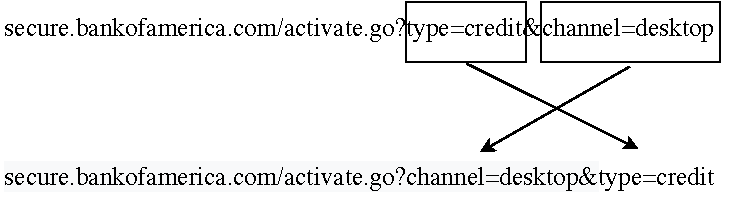
\includegraphics[width=0.75\linewidth]{urltran/figures/PermuteURL}
	\caption{An example of parameter reordering}
	\label{fig:urltran:permute_url}
\end{figure} 


 
